\chapter{\label{ch:neutrinophysics}Neutrino Physics} 

\minitoc

Despite being one of the most abundant particles in the universe, neutrinos are 
some of the most elusive; due to the fact that neutrinos can only interact via
the weak interaction. The history of neutrino physics is, therefore, strongly
connected to the discovery and study of weak interactions. Measurements by
Chadwick in 1914 showed that the energy spectrum of electrons released in
$\beta$--decays was continuous, this is in contrast to discrete spectra
observed in $\alpha$ and $\gamma$ decays, and seemingly violates
conservation of energy under the assumption of a two--body final state which was
expected at the time. In order to solve this problem, Pauli postulated that the 
continuous energy spectrum could be explained if the energy released in a 
$\beta$--decay could be shared with an additional neutral weakly interacting 
fermion, which Pauli named the neutron. Fermi later renamed Pauli's fermion to 
the neutrino, after Chadwick discovered the neutron in 1932. Despite claims 
that neutrinos might never be detected, not only have they now been discovered
but they have also been found to have a number of interesting properties, which 
were not anticipated when they were first postulated. 

This chapter will detail some of the history and theory of neutrinos and their 
interactions. Section \ref{nu_hist} will give a brief historical overview of 
neutrino physics. Section \ref{nu_sm} will introduce the theory of neutrinos 
in the Standard Model, followed by a discussion of neutrino oscillations in 
Section \ref{nu_osc}. Neutrino interactions will be discussed briefly in 
Section \ref{nu_prod}, and finally Section \ref{nu_sn} will discuss the 
production and measurement of neutrinos from supernovae.

\section{A Brief History of Neutrino Physics} \label{nu_hist}

The first attempt to incorporate the neutrino into a theoretical model came in
1934, when Fermi presented his theory of \(\beta\)--decay. In this theory, the 
neutrino takes part in a four--point interaction with the other components of 
the \(\beta\)--decay interaction\cite{Fermi1934}. The incredible success of 
this theory in explaining the observed properties of \(\beta\)--decays 
provided strong evidence for the neutrinos existence, however, in 1934 after 
using Fermi's theory to predict the strength of neutrino interactions, H. 
Bethe and R. Peierls found that the interactions were so weak that they might 
never be observed, a hypothesis that held true for over 20 
years\cite{Bethe1934}.

The first breakthrough in experimental neutrino physics would come in 1956, 
when F.  Reines and C. Cowan were attempting to measure positrons produced in 
inverse \(\beta\)--decay interactions,
\begin{equation*}
	\xoverline{\nu_e} + p \rightarrow n + e^+.
\end{equation*}
A detector containing 1400 litres of liquid scintillator was used to measure the
large flux of electron anti--neutrinos in the vicinity of the Savannah River 
nuclear reactor. They observed a large increase in the rate of positron events 
when the reactor was on compared to when the reactor was switched off. This 
was the first experimental evidence for the existence of 
neutrinos\cite{Reines1953}. 

The discovery of the electron neutrino gave rise to questions of neutrino 
flavour. As neutrinos are produced alongside a charged lepton it is natural to 
compare the properties of neutrinos with their partners in the weak 
interaction. At the time of the discovery of the neutrino there were two known 
charged leptons, the electron and the muon, and physicists questioned whether 
the neutrinos produced alongside muons are different from those produced 
alongside electrons. In 1962, Lederman et al discovered the muon neutrino at 
Brookhaven National Laboratory; by creating a beam of muon--associated 
neutrinos from decaying pions, and observing the leptons produced in neutrino 
interactions after all other particles had been absorbed. They found that only 
muons were produced in the resulting neutrino interactions and, therefore, 
the neutrinos produced were only ever associated with a muon. This showed that 
neutrinos are produced with a distinct flavour in weak 
interactions\cite{Danby1962}.

In 1973 the Gargamelle experiment at the European Organisation for Nuclear
Research (CERN) released results on the measurement of neutrino 
interactions\cite{Hasert1973}. They observed a new type of interaction, 
neutral current (NC) interactions, 
\begin{equation*}
	\nu_l + N \rightarrow \nu_l + X,
\end{equation*}
which are characterised by the lack of an observable charged lepton in the final
state. Unlike charged current (CC) interactions, which are mediated by the 
charged W boson, these NC interactions are mediated by the neutral 
\(\mbox{Z}^0\) boson.

With the discovery of the tau--lepton in 1977, it was expected that there should
be an associated tau neutrino, however, it wouldn't be detected until 2001 by 
the DONUT experiment\cite{Kodama2001}. In this experiment, tau neutrinos were 
produced from the decay of charmed mesons produced in collisions between 
protons and a stationary target. The neutrino interactions were detected in 
emulsion detectors, where the unique geometry of the interaction, in which a 
short tau track is produced at the vertex followed by a long muon track, 
allowed them to be distinguished from other 
decays.

While additional neutrino species are possible, data from measurements of the Z 
boson line--shape at the Large Electron--Positron Collider (LEP) in 1992 
restricts the number of active light neutrino species to three\cite{LEP1992}. 
An active light neutrino is any neutrino with \(m_\nu < \frac{m_Z}{2}\) that 
can interact with the Z boson, such that the decay \(Z \rightarrow \nu 
\xoverline{\nu} \) is possible.

Alongside the discovery of three different types of neutrino, there were
interesting results when observing neutrinos produced in the Sun. The flux of
neutrinos from the Sun at the Earth's surface had been predicted with Bachall's 
Standard Solar Model (SSM). However, in 1968 when Davis et al measured the 
flux in the Homestake experiment they found a deficit with respect to the 
prediction of the SSM\cite{Davis1968, Bahcall1968}, the so called solar 
neutrino problem. In the Homestake experiment, electron neutrinos were being 
measured via there inverse beta decay interactions with the chlorine in the 
target, 
\begin{equation*}
	v_e + ^{37}\mbox{Cl} \rightarrow ^{37}\mbox{Ar} + e^-.
\end{equation*}
The neutrino interaction rate was measured by counting the number of argon 
atoms in the chlorine tank, which was achieved by periodically bubbling helium
gas through the chamber to capture the argon atoms.

In addition to the solar neutrino problem, a similar deficit was observed in
1988 for muon neutrinos produced during cosmic--ray showers.  The Kamiokande 
experiment was able to measure both electron and muon neutrino interactions,
via the Cerenkov radiation produced by the charged leptons in water. The data
from Kamiokande was consistent with the expected rate of electron neutrinos 
from the atmosphere, however, a deficit of muon neutrinos was 
observed\cite{Hirata1988}. 

Super--Kamiokande, the next generation of the Kamiokande experiment, aimed to
understand the observed deficit of atmospheric muon neutrinos by using a larger 
water Cerenkov detector capable of resolving the angular distribution of 
atmospheric neutrino interactions. Super--Kamiokande consists of a cylindrical 
vessel containing 50 kt of ultra pure water, surrounded by an array of around 
13,000 photomultiplier tubes to detect the Cerenkov light. Electron and muon 
neutrinos can be distinguished based on the pattern of Cerenkov light that is 
left in the detector. Muons leave clear Cerenkov rings in the detector due to 
their higher mass, while electrons, which can scatter and shower, tend to leave 
diffuse \say{fuzzy} rings on the wall of the detector. In 1998, 
Super--Kamiokande published measurements of the flux of atmospheric muon 
neutrinos as a function of azimuthal angle\cite{Fukuda1998}. Since these 
neutrinos are created a short distance from the earths surface, their incoming 
angle can be used to estimate the distance travelled before they arrive at the 
detector. The down--going neutrinos have only travelled a short distance in 
the atmosphere (\(\sim 10 \mbox{km}\)), while the up--going neutrinos have 
travelled through the entire earth to reach the detector (\(\sim 13,000 
\mbox{km}\)). Figure \ref{fig:sk_flux}, shows the ratio of the measured flux 
to the prediction in the absence of oscillations, for neutrinos measured by 
Super Kamiokande as a function of \(\mbox{L} / \mbox{E}_\nu\). The muon 
neutrino flux is consistent with the no oscillation prediction at small 
\(\mbox{L} / \mbox{E}_\nu\), however, for large \(\mbox{L} / \mbox{E}_\nu\) a 
clear deficit is observed. 

\begin{figure}

	\centering

	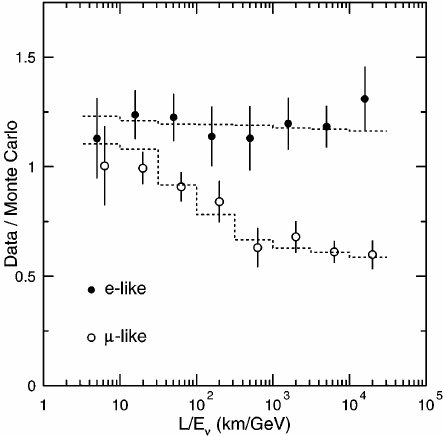
\includegraphics[width=0.7\textwidth]{figures/sk_flux.jpg}

	\caption
	[Ratio of data to Monte Carlo for electron and muon neutrino fluxes 
	measured by the Super Kamiokande experiment as a function of 
	\(\mbox{L} / \mbox{E}_\nu\).]
	{Ratio of data to Monte Carlo for electron and muon neutrino fluxes measured 
	by the Super Kamiokande experiment as a function of 
	\(\mbox{L} / \mbox{E}_\nu\). The Monte Carlo prediction is based on the
	assumption of no oscillations. The muon neutrino flux is consistent with the
	no oscillation prediction at small \(\mbox{L} / \mbox{E}_\nu\), however, for
	large \(\mbox{L} / \mbox{E}_\nu\) a clear deficit is observed. The best fit
	under the assumption of atmospheric (\(\nu_\mu \rightarrow \nu_\tau\))
	oscillations is shown, the best fit parameters are \(\Delta m^2 = 2.2 \times
	10^{-3} \mbox{eV}^2\), and \(\sin^22\theta = 1\). Figure from 
	\cite{Fukuda1998}.}
	\label{fig:sk_flux}

\end{figure}

While it couldn't isolate the exact cause of the solar neutrino problem, the
Sudbury Neutrino Observatory (SNO) was able to provide unique insight into the 
observed solar neutrino fluxes in 2002. Unlike other water Cerenkov detectors, 
SNO was filled with heavy water, \(\mbox{D}_2\mbox{O}\), instead of its 
lighter isotope. The use of heavy water gives rise to additional neutrino 
interactions, which allowed the SNO experiment to distinguish between three 
different interaction modes: charged current (CC), neutral current (NC), and 
elastic scattering (ES). Each mode is sensitive to different parts of the 
solar neutrino flux, including some sensitivity to the muon neutrino and tau 
neutrino fluxes via the NC and ES interactions. Analysis of the data for each 
of the three unique interaction modes led to a measurement of the flavour 
composition of the solar neutrino flux at earth, whilst also finding the 
overall neutrino flux at earth to be consistent with the SSM.  Figure 
\ref{fig:sno_flux} shows the composition of the solar neutrino flux as 
measured in the SNO experiment\cite{Ahmad2002}, the flux prediction based on 
the measured rate of NC events is consistent with the predictions of the SSM. 
The composition of solar neutrinos measured in the SNO experiment is not a 
result of simple neutrino oscillations, it also depends on the effect of matter 
on the neutrino propagation in the Sun, via the Mikheyev–Smirnov–Wolfenstein 
(MSW) effect. However, at the time a number of solutions were still considered 
possible: MSW conversion, decoherence, neutrino decay, and 
others\cite{Smirnov:2016xzf}. 

\begin{figure}

	\centering

	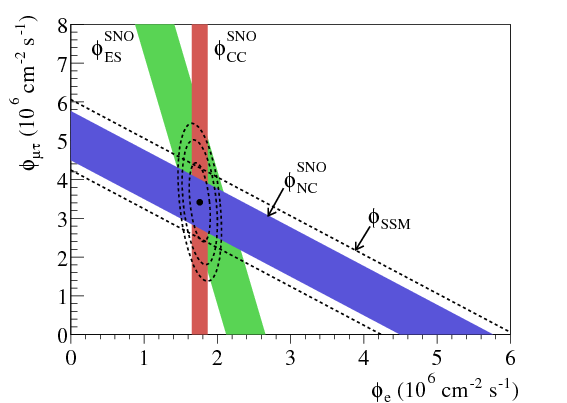
\includegraphics[width=0.8\textwidth]{figures/sno_flux.png}

	\caption
	[Solar neutrino flux composition as measured by the SNO experiment.]
	{Solar neutrino flux composition as measured by the SNO experiment. The
	coloured bands represent the measured flux of charged current (CC),
	neutral current (NC), and elastic scattering (ES) events, including a \(\pm 1
	\sigma\) spread. The central contours represent 68\%, 95\%, and 99\%
	probability contours for the joint \(\phi_e\) and \(\phi_{\mu \tau}\) fit. The
	dashed lines represent the predicted flux of \(^8\mbox{B}\) neutrinos based on
	the standard solar model. Figure from \cite{Ahmad2002}. }

	\label{fig:sno_flux}

\end{figure}

An \(\mbox{L/E}_\nu\) dependence in the neutrino flux would have to be measured 
in order to prove that neutrino oscillations are unique solution to the problem.
This measurement would require a much shorter baseline, and a detector with a
good energy resolution, which would be provided by the Kamioka Liquid
Scintillator Anti--neutrino Detector (KamLAND). In 2002, the experiment 
measured \(\xoverline{\nu_e}\) oscillations from a number of nuclear reactors, 
which produce neutrinos at the MeV scale\cite{ Eguchi2003, Araki2005}. Along 
with an overall deficit of neutrino events, they were able to use the high 
energy resolution of the KamLAND detector to measure an \(\mbox{L/E}_\nu\) 
dependence of the \(\xoverline{\nu_e}\) survival probability.  Figure 
\ref{fig:kamland_spectrum} shows the ratio of the observed neutrino flux to 
the no oscillation predicted flux as a function of \(\mbox{L/E}_\nu\). A clear 
dependence can be seen and this data was enough to prove that neutrino 
oscillations were the only solution to the solar neutrino problem.  

\begin{figure}

	\centering

	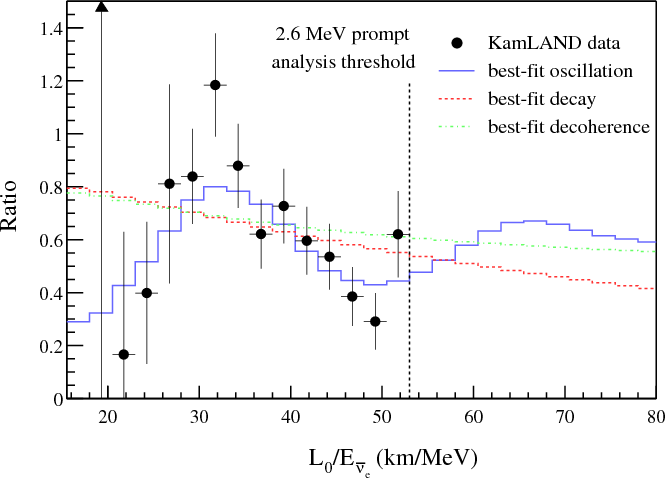
\includegraphics[width=0.8\textwidth]{figures/kamland_spec.png}

	\caption
	[Ratio of observed neutrino flux to the predicted flux in the absence of
	neutrino oscillations in the KamLAND experiment.]
	{Ratio of observed neutrino flux to the predicted flux in the absence of
	neutrino oscillations in the KamLAND experiment as a function of 
	\(\mbox{L/E}_\nu\). The data is fit with three different models: the red 
	dashed line represents the best fit to a neutrino decay model, the green 
	dashed line is for a decoherence model, and the solid blue line represents the 
	best fit of the data to a neutrino oscillation model. The neutrino oscillation
	model, which has a different shape to the other two models, is found to give 
	the best fit to the data. Figure from \cite{Araki2005}.} 

	\label{fig:kamland_spectrum}

\end{figure}

Based on the results of the above experiments, it was assumed that electron and
muon type neutrinos oscillate into tau type neutrinos, which go undetected. 
The first evidence of tau neutrino production in oscillations wouldn't come 
until 2010, when the OPERA experiment measured a \(\nu_\tau\) candidate in a 
\(\nu_\mu\) beam. They used similar emulsion detectors to those used to 
discover the \(\nu_\tau\) in DONUT, and a muon neutrino beam on a 730 km 
baseline from CERN to Laboratori Nazionali del Gran Sasso (LNGS). By the end 
of the experiment a total of 10 candidate events have been observed, 6.1 
\(\sigma\) above the expected background\cite{Agafonova2010, Agafonova2018}.

Since the discovery of neutrino oscillations, many more experiments have made
measurements of oscillations, and the majority of the parameters of the neutrino
oscillation models have been constrained. Important results of these 
experiments for constraining the parameters of the neutrino oscillation models 
will be highlighted in Section \ref{nu_osc}, along with a theoretical overview 
of neutrino oscillations.

\section{Neutrinos in the Standard Model} \label{nu_sm}

In the standard model, neutrinos form part of the left handed fermion doublets,
\begin{equation*}
	\psi_i = \begin{pmatrix}[1.5] \nu_i \\ l^-_i \end{pmatrix},
\end{equation*}
where they are paired with a charged lepton of the same flavour in
CC interactions, and $i$ represents any of the three known generations of 
leptons. Their interaction with other particles in the standard model is
determined by the electroweak theory, which is derived from the $SU(2)
\times U(1)$ gauge group. The neutrino fields enter into the SM Lagrangian in
the CC and NC interactions:
\begin{align}
	\label{eqn:cc_lag}
	\mathcal{L}^{CC} &= -\frac{g_W}{\sqrt{2}}\; j^{CC}_\alpha(x)\; W^\alpha(x)\; +\; h.c. \nonumber \\
	\mathcal{L}^{NC} &= -\frac{g_W}{cos\theta_W}\; j^{NC}_\alpha(x)\; Z^\alpha(x)\; +\; h.c.
\end{align}
Here 
\begin{equation*}
	j^{CC}_{\alpha}(x) = \sum_{\beta=e,\mu,\tau} \xoverline{\nu_\beta}(x)\;
	\gamma_{\alpha} \; \frac{1}{2} \left(1 - \gamma^5 \right) l_\beta(x)
\end{equation*}
is the leptonic charged--current, and
\begin{equation*}
	j^{NC}_{\alpha}(x) = \frac{1}{2} \sum_{\beta=e,\mu,\tau} \xoverline{\nu_\beta}(x)\;
	\gamma_{\alpha}\; \frac{1}{2} \left(1 - \gamma^5 \right)  \nu_\beta(x)
\end{equation*}
is the neutrino neutral--current, $W^\alpha(x)$ and $Z^\alpha(x)$ are the vector
boson fields for the $W^\pm$ and $Z^0$ bosons respectively, $g_W$ is the 
electroweak coupling constant, and $\theta_W$ is the Weinberg angle.

Mass is included in the standard model through the Dirac mass term in the
Lagrangian,
\begin{align*}
	\mathcal{L}^{D} &= m_D \xoverline{\psi} \psi \nonumber \\
	&= m_D \overline{(\psi_L + \psi_R)}(\psi_L + \psi_R) \nonumber \\ 
	&= m_D(\xoverline{\psi}_L \psi_R + \xoverline{\psi}_R \psi_L),
\end{align*}
where $L$ and $R$ represent the left and right handed components of the field.
The lack of right handed neutrino states means that neutrinos are assumed 
to be massless in the standard model. For massive neutrinos to exists in the 
standard model, right handed neutrino fields need to be introduced. In addition, 
it is still not known whether neutrinos are Dirac or Majorana particles, meaning that 
additional Majorana mass terms are possible. A more general neutrino mass term 
including both Dirac and Majorana components is 
\begin{equation}
	\label{eqn:m_dirac_majorana}
	\mathcal{L}^{D+M} = 
	\begin{pmatrix}[1.5] \xoverline{\nu}_L \; \xoverline{\nu}_R \end{pmatrix} 
	\begin{pmatrix}[1.5] m_L \; m_D \\ m_D \; m_R \end{pmatrix} 
	\begin{pmatrix}[1.5] \nu_L \\ \nu_R \end{pmatrix}.
\end{equation}

\section{Neutrino Oscillations} \label{nu_osc}

Neutrino oscillations are a result of quantum mechanical interference between
different massive neutrino eigenstates. Neutrinos are produced in a state of 
definite flavour, \(\alpha = e, \mu, \tau\), in charged current (CC) and 
neutral current (NC) weak interactions, 
\begin{equation*}
	W^+ \rightarrow l_\alpha^+ \nu_\alpha, \quad  W^- \rightarrow l^-_\alpha \nu_\alpha, \quad  Z   \rightarrow \nu_\alpha \xoverline{\nu_\alpha}.
\end{equation*}
The CC processes are used in neutrino oscillation experiments because
they give information about the initial flavour state of the neutrinos. These
processes are governed by the Lagrangian of the CC leptonic interactions, as in
Equation \ref{eqn:cc_lag}.

Neutrino flavour states, $\nu_\alpha$, can be represented as a superposition of 
neutrino mass eigenstates in the form,
\begin{equation}
	\label{eqn:mass_sup}
	\nu_\alpha = \sum_{k} U^*_{\alpha k} \nu_k,
\end{equation}
where $\nu_k$ are the neutrino mass eigenstates, and U is a unitary mixing
matrix. 

The representation of neutrino flavour states as a superposition of mass 
eigenstates gives rise to the phenomenon of neutrino oscillations. Consider a 
neutrino produced in a CC weak interaction with flavour \(\alpha\). 
This neutrino flavour state is described by equation \ref{eqn:mass_sup},
where \(U\) is a unitary mixing matrix called the PMNS 
(Pontecorvo, Maki, Nakagawa, and Sakata) matrix. For three flavour mixing the 
PMNS matrix takes the form:
\begin{equation*}
	U = 
	\begin{pmatrix}[2]
		U_{e1} & U_{e2} & U_{e3} \\
		U_{\mu1} & U_{\mu2} & U_{\mu3} \\
		U_{\tau1} & U_{\tau2} & U_{\tau3} \\
	\end{pmatrix}.
\end{equation*}

\subsection{Neutrino Oscillations in Vacuum}
In a vacuum, the neutrino mass states are eigenstates of the free particle Hamiltonian
\begin{equation*}
	{\cal H} \ket{\nu_k} = E_k \ket{\nu_k},
\end{equation*}
with energy
\begin{equation*}
	E_k = \sqrt{\vb{p}^2 + m_k^2}.
\end{equation*}
So the solutions to the time dependent Schrodinger equation are plane waves
\begin{equation*}
	\ket{\nu_k(t)} = e^{-iE_kt}\ket{\nu_k}.
\end{equation*}
The time evolution of the initial flavour state is:
\begin{equation}
	\label{eqn:flavour_time_mass}
	\ket{\nu_\alpha(t)} = \sum_k U_{\alpha k}^* e^{-iE_kt} \ket{\nu_k}.
\end{equation}

The mass states can be written in terms of the flavour states by inverting
Equation \ref{eqn:mass_sup},
\begin{equation}
	\label{eqn:flav_sup}
	\ket{\nu_k} = \sum_\alpha U_{\alpha k} \ket{\nu_\alpha},
\end{equation}
where, we have used the fact that the states form an orthonormal basis,
\(\braket{\nu_\alpha}{\nu_\beta} = \delta_{\alpha \beta}\), and that the 
transformation matrix is unitary, \(UU^\dagger = \vb{1}\).

Substituting Equation \ref{eqn:flav_sup} into the time evolution of the flavour
state, Equation \ref{eqn:flavour_time_mass}, gives:
\begin{equation*}
	\ket{\nu_\alpha(t)} = \sum_{\beta = e, \mu, \tau} \left(\sum_k
	U^*_{\alpha k} e^{-iE_kt} U_{\beta k} \right) \ket{\nu_{\beta}} 
\end{equation*}
So as the initial flavour state evolves with time, it becomes a superposition 
of different flavour states; this process is known as neutrino oscillation.
The probability of finding the initial neutrino in flavour state \(\nu_\beta\) 
as a function of time is:
\begin{align}
	\label{eqn:p_osc_u}
	P_{\nu_\alpha \rightarrow \nu_\beta}(t) &= \abs{\braket{\nu_\beta}{\nu_\alpha(t)}}^2 \nonumber \\
	                                        &= \sum_{kj} U^*_{\alpha k} U_{\beta k} U_{\alpha j} U^*_{\beta j} e^{-i(E_k - E_j)t}.
\end{align}

All neutrino oscillation experiments to date operate in a regime where 
\(E \gg m\), in this regime the relativistic energy relation for neutrinos can 
be expanded as \({E_k \simeq E + \frac{m_k^2}{2E}}\), where \(E = \abs{p}\). 
Hence, 
\begin{equation*}
	E_k - E_j \simeq \frac{m_k^2 - m_j^2}{2E} = \frac{\Delta m_{kj}^2}{2E}.
\end{equation*}
Another modification to the formula is a result of the fact that neutrino 
oscillation experiments do not measure the neutrino propagation time, \(t\). 
Instead, they measure the propagation distance, \(L\), also known as the 
baseline. In the ultra--relativistic limit, \({t \simeq L}\) in natural units,
and as a result, Equation \ref{eqn:p_osc_u} can be approximated as:
\begin{equation*}
	P_{\nu_\alpha \rightarrow \nu_\beta}(t) = \sum_{kj} U^*_{\alpha k} U_{\beta k} U_{\alpha j} U^*_{\beta j} e^{-i\frac{\Delta m^2_{kj}L}{2E}}.
\end{equation*}

Splitting the sum into its real and imaginary parts emphasises the possibility
of charge--parity (CP) violation in neutrino oscillations. CP--violation occurs if the imaginary
component of the matrix product is none--zero. 
\begin{align*}
	P_{\nu_\alpha \rightarrow \nu_\beta}(t) = \delta_{\alpha \beta} 
	&- 4 \sum_{j > k} \operatorname{Re}(U^*_{\alpha k} U_{\beta k} U_{\alpha j} U^*_{\beta j}) \sin^2(\frac{\Delta m^2_{kj} L}{2E}) \nonumber \\
	&\pm 2 \sum_{j > k} \operatorname{Im}(U^*_{\alpha k} U_{\beta k} U_{\alpha j} U^*_{\beta j}) \sin^2(\frac{\Delta m^2_{kj} L}{2E}).
\end{align*}
The third term here is responsible for CP violation in neutrino oscillations,
the positive case corresponds to neutrinos and the negative case to
anti--neutrinos.

The probability of oscillation is, therefore, dependent on properties determined
by nature, in the form of PMNS matrix elements and mass squared differences, and
those which can be chosen by experiments, the distance travelled, L, and the
neutrino energy, E. In a vacuum, the oscillation probability is only dependent 
on the magnitude of the squared mass difference between the neutrino mass
eigenstates. There is no information about the absolute masses of the 
neutrino eigenstates or their ordering in neutrino oscillations and, therefore,
the question of the absolute neutrino masses cannot be answered with neutrino 
oscillation experiments. To get access to the absolute masses other 
experiments are required, e.g. direct mass measurements with tritium beta 
decay experiments such as KATRIN\cite{Aker:2019qfn}. Neutrino oscillation 
experiments can give insight on the ordering of the neutrino masses, but
the oscillations of neutrinos in matter must be considered in order to achieve
this.

\subsection{Neutrino Oscillations in Matter}
In real neutrino oscillation experiments, neutrinos travel through matter,
whether it be the matter in a star or the earths crust. Neutrinos propagating in
matter are subject to an additional potential due to the interaction of the 
neutrinos with the electrons and nucleons in the medium.  This interaction can 
significantly modify the flavour of the beam relative to oscillations in 
vacuum.

In matter, neutrinos can scatter off particles by interacting with either
the charged--current or neutral--current interactions, as shown in Figure
\ref{fig:nu_in_matter}. These interactions give rise to additional effective
potentials, which the neutrinos experience while they are travelling,
\begin{align*}
	V_{CC} &= \sqrt{2} G_F N_e, \\
	V_{NC}^f &= \sqrt{2} G_F N_f g_V^f,
\end{align*}
where $G_F$ is the Fermi weak coupling constant, $N_e$ and $N_f$ are the number
densities of electrons and other fermions respectively, and $g_V^f$ is the
vector coupling constant for a given fermion f.
\begin{figure}
	\centering

	\begin{subfigure}[b]{0.49\textwidth}
		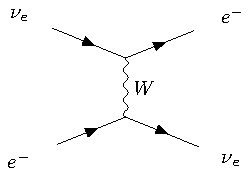
\includegraphics[width=\textwidth]{latex_extras/ne_cc.pdf}
		\caption{Charged current scattering.}
		\label{fig:nu_cc}
	\end{subfigure}
	\hfill
	\begin{subfigure}[b]{0.49\textwidth}
		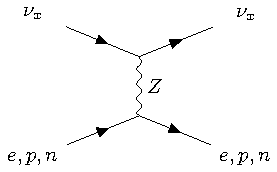
\includegraphics[width=\textwidth]{latex_extras/n_nc.pdf}
		\caption{Neutral current scattering.}
		\label{fig:nu_nc}
	\end{subfigure}

	\caption
	[Feynman diagrams for neutrino scattering in matter.]
	{Feynman diagrams for neutrino scattering in matter via a charge current and a
	neutral current process.}

	\label{fig:nu_in_matter}
\end{figure}

Neutral--current scattering is independent of neutrino flavour, meaning that
the additional potential does not affect oscillations. However, the charged
current potential is only present for $\nu_e$ and, therefore, it will impact the
mass eigenstates by different amounts depending on their relative $\nu_e$
component.

A full description of the effects of matter on neutrino oscillations is outside
the scope of this thesis, although it is discussed at length in other sources
such as \cite{GiuntiCarlo2007FoNP}. For the purposes of this thesis, it is
sufficient to note that the propagation of neutrinos in matter changes the
oscillations probabilities, and that this must be taken into account by 
oscillation experiments.

One implication of the effects of matter on oscillations is that it introduces
sensitivity to the sign of the mass splittings\cite{GiuntiCarlo2007FoNP}, 
allowing experiments to determine the relative ordering of the neutrino 
masses. By considering the pattern of neutrino oscillations in the sun it is 
possible to determine that $\Delta m_{21}^2 > 0$\cite{PhysRevD.98.030001}. 
The sign of the remaining mass splitting, $\Delta m_{32}^2$, remains unknown,
which leaves two possibilities for the ordering of neutrino masses. Normal 
ordering (NO), in which $m_3 > m_2 > m_1$, and inverted ordering (IO), where $m_2 > m_1 
> m_3$, which are depicted in Figure \ref{fig:mass_ordering}. 
\begin{figure}
	\centering
	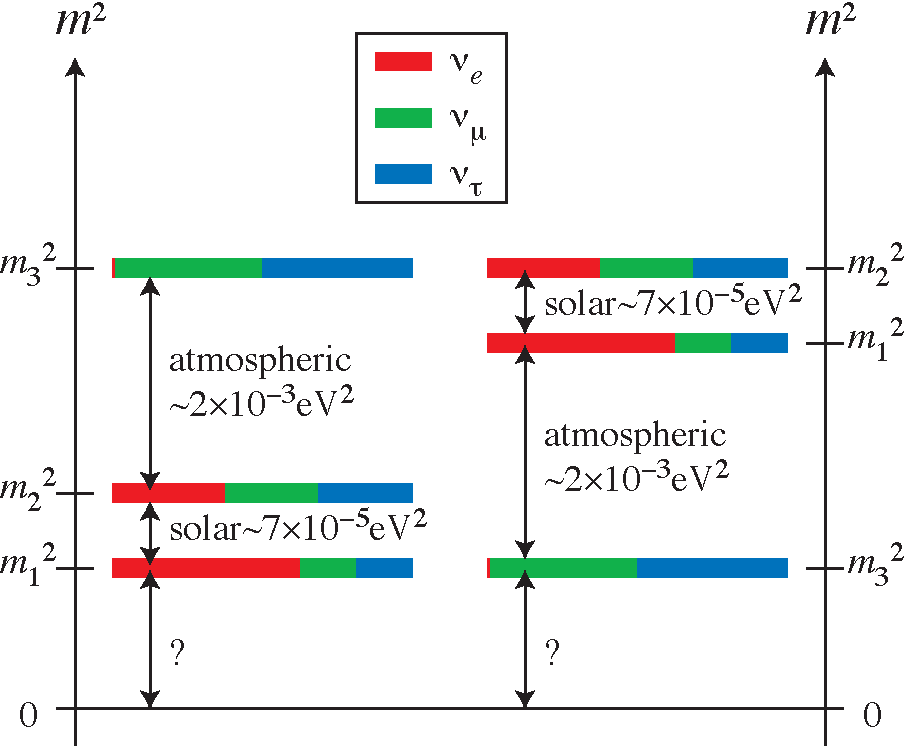
\includegraphics[width=0.7\textwidth]{figures/mass.pdf}
	\caption
	[The two possible neutrino mass orderings.]
	{The two possible neutrino mass orderings. Left: normal ordering. Right: 
	inverted ordering.  Figure from \cite{SKing}.}
	\label{fig:mass_ordering}
\end{figure}

\subsection{Current Knowledge and Open Questions}

At the time of writing, the most widely accepted model of neutrino oscillations
involves three neutrino mass eigenstates. In this model, the PMNS matrix is 
often parametrised in terms of three mixing angles \(\theta_{12}\), 
\(\theta_{13}\), and \(\theta_{23}\) and three CP--violating phases 
\dcp{}, \(\alpha_1\), and \(\alpha_2\):
\begin{equation*}
	U = 
	\underbrace{\begin{pmatrix}[2] 
		c_{12}  & s_{12} & 0 \\
		-s_{12} & c_{12} & 0 \\
		0       & 0      & 1 \\
	\end{pmatrix}}_{\mbox{\small Solar}}
	\underbrace{\begin{pmatrix}[2]
		c_{13}                 & 0 & s_{13}e^{-i\delta_{CP}} \\
		0                      & 1 & 0 \\
		-s_{13}e^{i\delta_{CP}} & 0 & c_{13} \\
	\end{pmatrix}}_{\mbox{\small Cross--mixing}}
	\underbrace{\begin{pmatrix}[2]
		1 & 0       & 0 \\
		0 & c_{23}  & s_{23} \\
		0 & -s_{23} & c_{23} \\
	\end{pmatrix}}_{\mbox{\small Atmospheric}}
	\underbrace{\begin{pmatrix}[2]
		e^{i\frac{\alpha_1}{2}} & 0                       & 0 \\
		0                       & e^{i\frac{\alpha_2}{2}} & 0 \\
		0                       & 0                       & 1 \\
	\end{pmatrix}}_{\mbox{\small Majorana}}.
\end{equation*}
Expressing the mixing matrix like this, factorises the matrix into its 
components, which are responsible for oscillations in different regimes. 
The Solar mixing matrix contains only \(\theta_{12}\) which is dominant in Solar
neutrino oscillations, and the Atmospheric mixing matrix, which dominates in the mixing of 
atmospheric neutrinos, and is a function of \(\theta_{23}\). The final component
that has an impact on neutrino oscillations, is the cross--mixing matrix or 
reactor matrix, which depends on the final mixing angle, \(\theta_{13}\), and 
on one of the CP--violating phases, \dcp{}. If \dcp{} is non--zero, then U 
will have complex components in off diagonal elements, leading to different 
probabilities for CP flipped oscillations, \(P(\nu_\alpha \rightarrow 
\nu_\beta) \neq P(\xoverline{\nu_\alpha} \rightarrow \xoverline{\nu_\beta})\). 
Discovery of this effect, which is known as CP--violation,  is one of the 
major goals of the next generation of neutrino oscillation experiments.

The final matrix in the factorised version of the PMNS matrix is called the 
Majorana component. The CP--violating phases in this matrix cancel out in the 
oscillation probability, and so they can't be measured in neutrino oscillation 
experiments.  In fact, they only lead to physical effects if neutrinos are 
Majorana particles (i.e. if they are their own antiparticle). Other experiments 
are required to determine if neutrinos are Majorana particles, for example, 
neutrinoless double beta decay experiments such as CUORE\cite{Arnaboldi2004}, 
NEXT\cite{Alvarez2012}, and SNO+\cite{Andringa2016}. The question of the 
nature of neutrinos has implications on neutrino mass generation, as mentioned 
in Equation \ref{eqn:m_dirac_majorana}.

A large number of neutrino oscillation measurements have now been made by
solar, reactor, atmospheric, and accelerator neutrino experiments. When
combined, the results of these experiments give us our best estimates of 
neutrino oscillation parameters. The latest combined results, from the 2019 
Nu--Fit global neutrino oscillation analysis\cite{Esteban:2018azc} are 
summarised below.  Each measurement is given for both the normal hierarchy and 
the inverted hierarchy cases, and the major contributing experiments are
highlighted in each case.

\subsubsection*{$\boldsymbol{\theta_{12}}$}

The constraints on the solar mixing angle, $\theta_{12}$, are dominated by a
combination of data from solar neutrino experiments, such as SNO\cite{Ahmad2002}
and Super Kamiokande\cite{PhysRevLett.86.5651}, with data from the KamLAND 
experiment\cite{Araki2005}. The current constraint is,
\begin{align*}
	\sin^2(\theta_{12}) &= 0.310 \mbox{ } \substack{+ 0.013 \\ - 0.012} \quad \mbox{(NO)} \\
	                    &= 0.310 \mbox{ } \substack{+ 0.013 \\ - 0.012} \quad \mbox{(IO)}
\end{align*}

\subsubsection*{$\boldsymbol{\Delta m^2_{21}}$}

The best measurement of $\Delta m^2_{21}$ is also dominated by a combination of
solar neutrino data with the results from KamLAND. The measured value is,
\begin{align*}
	\Delta m^2_{21} &= (7.39 \mbox{ } \substack{+ 0.21 \\ - 0.20}) \times 10^{-5} \mbox{  eV}^2 \quad \mbox{(NO)} \\
	                &= (7.39 \mbox{ } \substack{+ 0.21 \\ - 0.20}) \times 10^{-5} \mbox{  eV}^2 \quad \mbox{(IO)} \\
\end{align*}

\subsubsection*{$\boldsymbol{\theta_{23}}$ and $\boldsymbol{\Delta m^2_{32}}$}

There is a strong correlation between $\theta_{23}$ and $\Delta m^2_{32}$ and,
therefore, their measurements are usually presented as a two--dimensional
contour. Figure \ref{fig:delm_sin23} shows a comparison of the world--leading
contours for $\sin^2 (\theta_{23})$--$\Delta m^2_{32}$, with the tightest error
bands coming from long baseline accelerator experiments such as T2K, MINOS, and 
\nova{}\cite{PhysRevD.96.092006, PhysRevLett.112.191801, PhysRevLett.123.151803}. 
The results are dependent on the neutrino mass ordering; based on the Nu--Fit 
global three neutrino oscillation analysis\cite{Esteban:2018azc}, 
\begin{align*}
	|\Delta m^2_{32}| &= (+ 2.525 \mbox{ } \substack{+ 0.033 \\ - 0.031}) \times 10^{-3} \mbox{  eV}^2 \quad \mbox{(NO)} \\
	                  &= (- 2.512 \mbox{ } \substack{+ 0.034 \\ - 0.031}) \times 10^{-3} \mbox{  eV}^2 \quad \mbox{(IO)},
\end{align*}
and 
\begin{align*}
	\sin^2(\theta_{23}) &= 0.582 \mbox{  } \substack{+ 0.015 \\ - 0.019} \quad \mbox{(NO)} \nonumber \\
	                    &= 0.582 \mbox{  } \substack{+ 0.015 \\ - 0.018} \quad \mbox{(IO)}.
\end{align*}

\begin{figure}
	\centering
	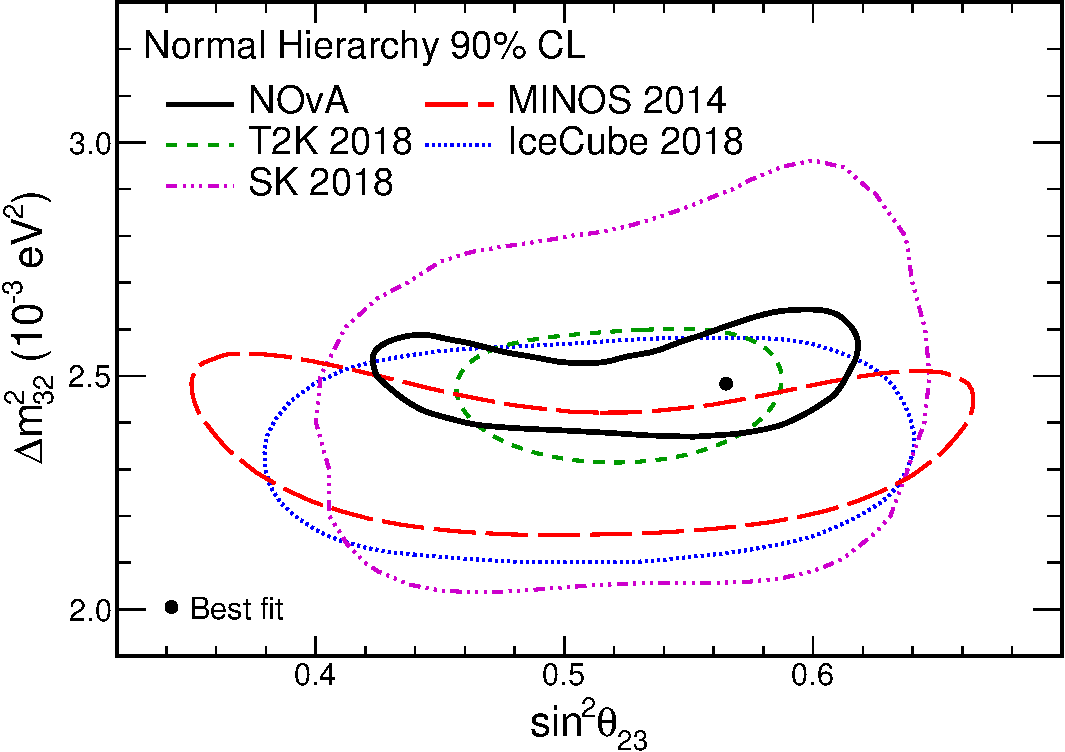
\includegraphics[width=0.9\textwidth]{figures/theta23_msquare.pdf}
	\caption 
	[90\% confidence intervals for $\sin^2 (\theta_{23})$--$\Delta m^2_{32}$ from
	a number of leading neutrino oscillation experiments.]
	{The 90\% confidence region contours for 
	$\sin^2 (\theta_{23})$--$\Delta m^2_{32}$ from a number of the leading 
	neutrino oscillation experiments\cite{PhysRevD.96.092006, PhysRevLett.112.191801, PhysRevLett.123.151803}. 
	The best fit point for the \nova{} experiment is shown as a black dot.  
	Figure from \cite{PhysRevLett.123.151803}.}
	\label{fig:delm_sin23}
\end{figure}

\subsubsection*{$\boldsymbol{\theta_{13}}$}
Reactor neutrino experiments such as Daya Bay\cite{An:2012eh}, Double 
Chooz\cite{Abe:2013sxa}, and RENO\cite{Ahn:2012nd} have made precise
measurements of $\theta_{13}$, as well as some long baseline oscillation 
experiments, such as T2K and \nova{}. The Nu--Fit three neutrino global fit to 
the reactor data gives,
\begin{align*}
	\sin^2 \theta_{13} &= 0.02240 \substack{+ 0.00065 \\ - 0.00066} \quad \mbox{(NO)} \\ .
	                   &= 0.02263 \substack{+ 0.00065 \\ - 0.00066} \quad \mbox{(IO)}  
\end{align*}

\subsubsection*{Mass Ordering}
The long baseline oscillation experiments T2K and \nova{} have both shown a
preference for normal mass 
ordering\cite{PhysRevD.96.092006,PhysRevLett.123.151803}. When these results are
combined in the Nu--Fit three--neutrino oscillation analysis, inverted 
ordering is currently disfavoured with a $\Delta \chi^2 = 9.3$.

\subsubsection*{$\boldsymbol{\delta_{CP}}$}
While there are no accurate measurements of \dcp{} there are some hints, from
long baseline accelerator neutrino experiments T2K and \nova{}, that it
may be none--zero. These limits are based on joint fits to four data samples: 
electron neutrino appearance, electron anti--neutrino appearance, muon 
neutrino disappearance, and muon anti--neutrino disappearance.

The T2K experiment's joint fit shows an excess of electron neutrino events, and 
a deficit of anti--electron neutrino events, when compared to the predictions 
for \(\delta_{CP} = 0\). This results in a preference for negative values of 
\dcp{} with a \(3\sigma\) confidence interval of \([-3.41, -0.03]\) in the 
case of normal neutrino mass ordering. The results of the T2K fit are shown 
in Figure \ref{fig:t2k_cp}\cite{Abe2019}.

\begin{figure}
	\centering
	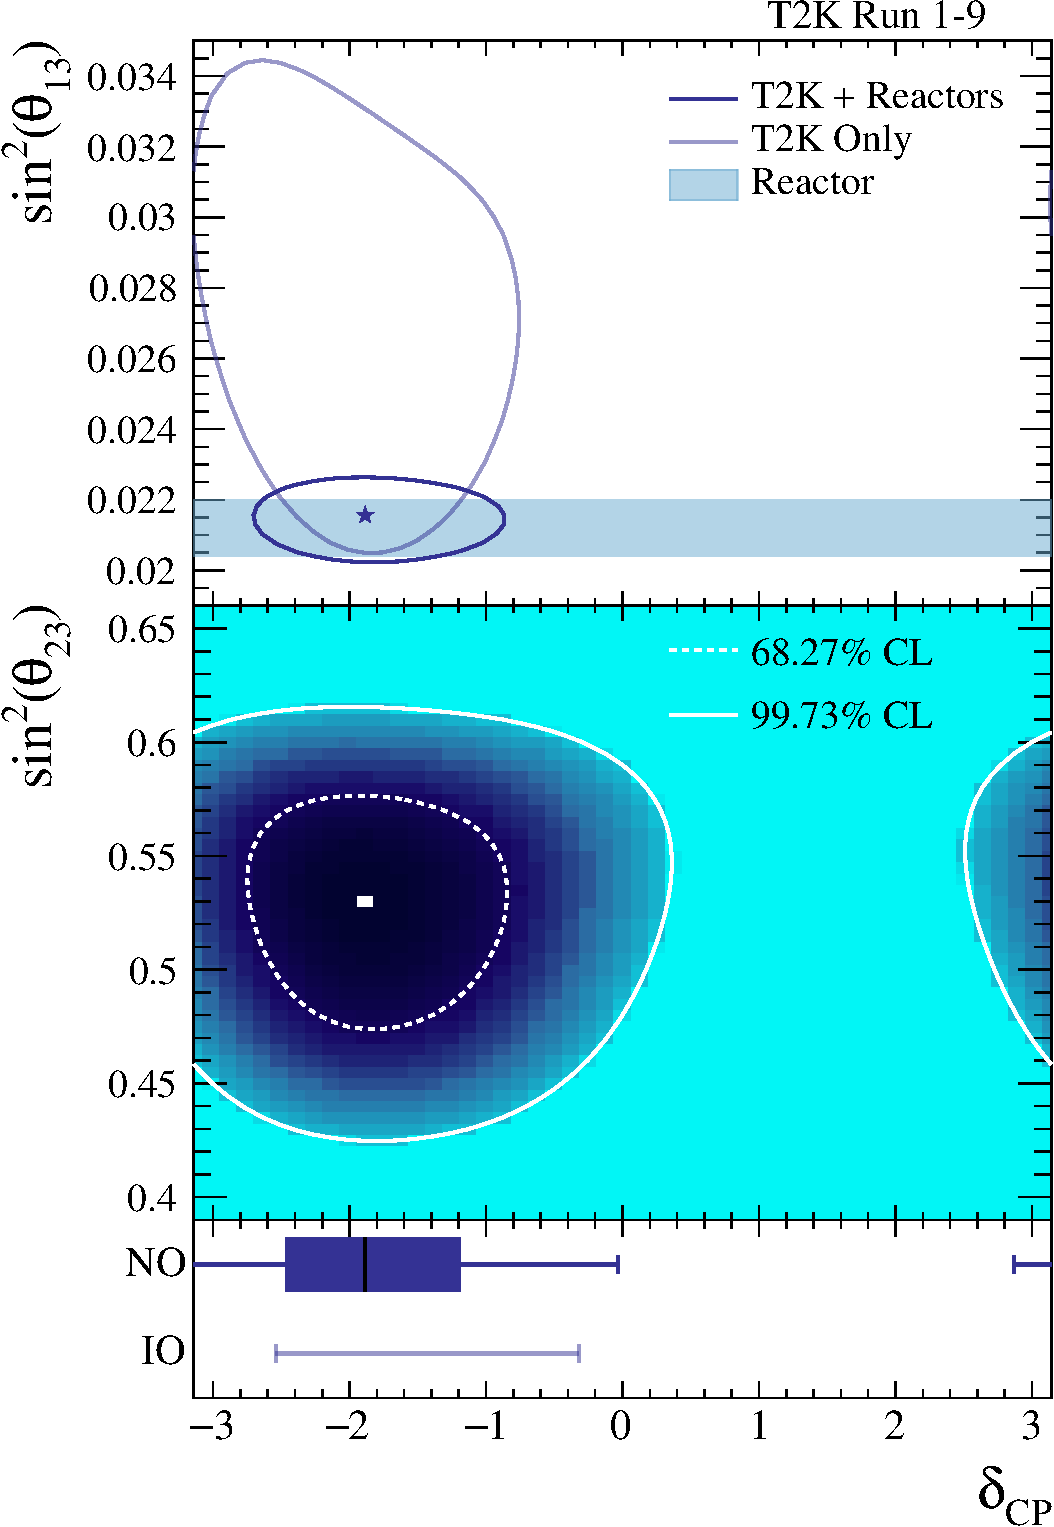
\includegraphics[height=0.75\textheight]{figures/t2k_cp.pdf}
	\caption
	[Confidence intervals for \dcp{} from the T2K experiment.]
	{Confidence intervals for \dcp{} from the T2K experiment. Figure from 
	\cite{Abe2019}. 

	\medskip
	\textbf{Top:} 68.27\% confidence level contours for \dcp{} versus $\sin^2\theta_{13}$ 
	under the assumption of normal ordering.

	\medskip
	\textbf{Middle:} Confidence intervals at the 68.27\% and 99.73\% confidence level for 
	\dcp{} versus $sin^2\theta_{23}$ from a fit to T2K and reactor data under the 
	assumption of normal ordering.

	\medskip
	\textbf{Bottom:} Confidence intervals for \dcp{} from a fit to T2K and reactor data for 
	both the normal and inverted orderings. The vertical line in the shaded box 
	shows the best-fit value of \dcp{}, the shaded box shows the 68.27\% 
	confidence interval, and the error bar shows the 99.73\% confidence interval. 
	}

	\label{fig:t2k_cp}

\end{figure}

The \nova{} experiment has also performed joint fits to neutrino and
anti--neutrino oscillation data, the results of the fit are shown in Fig.
\ref{fig:nova_cp}. As with T2K, the normal mass ordering is preferred, however,
for \nova{} the full range of \dcp{} is covered at $3\sigma$, highlighting the 
need for further study of CP--violation in neutrino 
oscillations\cite{PhysRevLett.123.151803}.

\begin{figure}

	\centering

	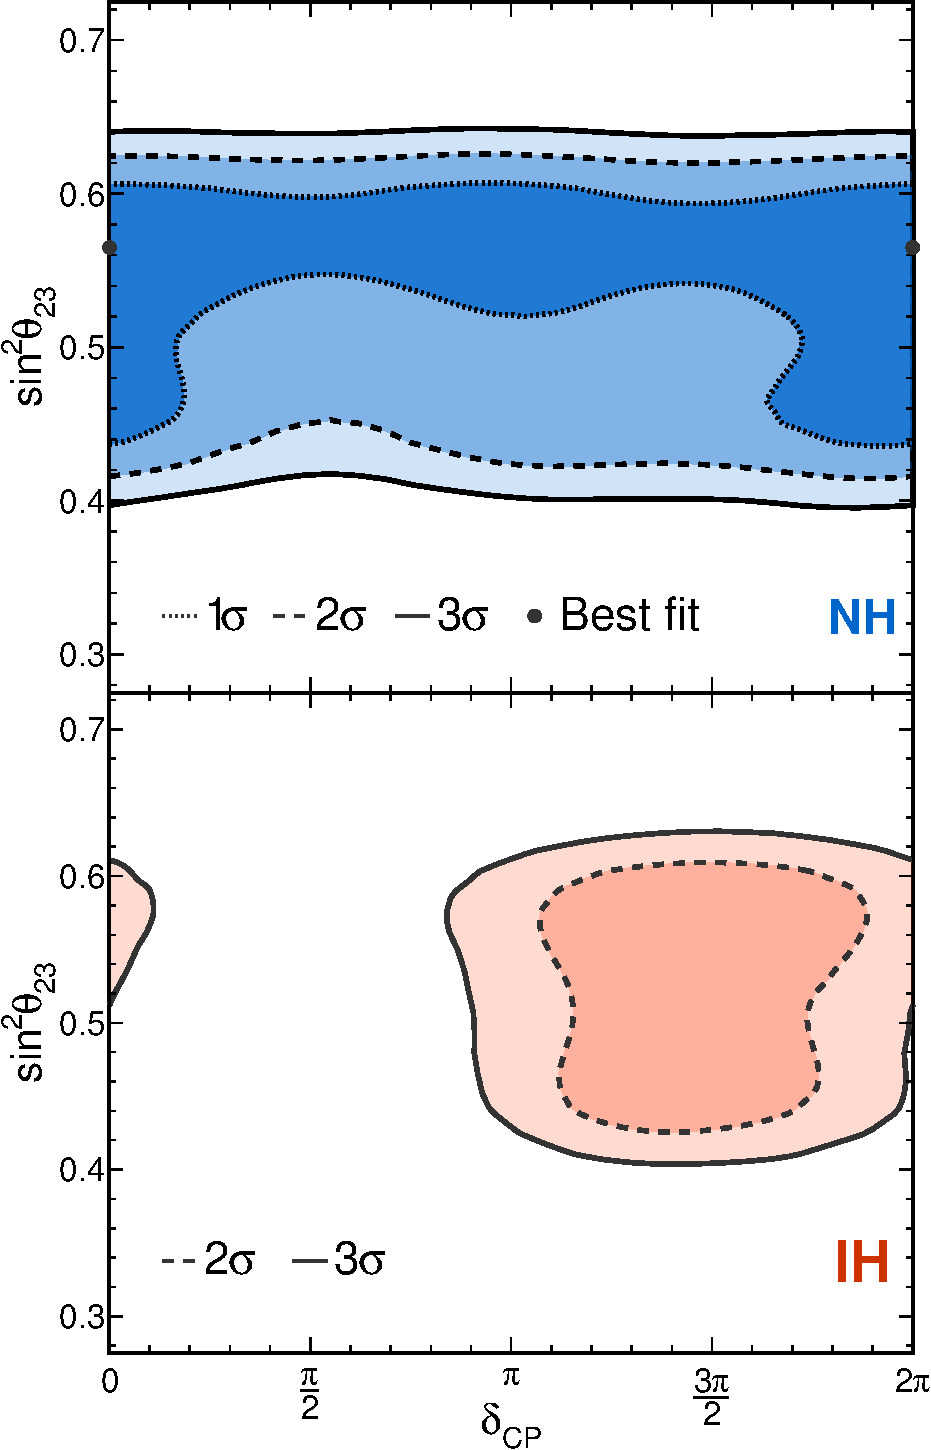
\includegraphics[height=0.75\textheight]{figures/nova_dcp.pdf}

	\caption
	[Confidence intervals for \dcp{} from the \nova{} experiment.]
	{Confidence intervals for \dcp{} from the \nova{} experiment. Figure from 
	\cite{PhysRevLett.123.151803}.

	\medskip
	\textbf{Top:} Confidence interval for \dcp{} versus $\sin^2\theta_{23}$ under the
	assumption of normal ordering.

	\medskip
	\textbf{Bottom:} Confidence interval for \dcp{} versus $\sin^2\theta_{23}$ under the
	assumption of inverted ordering.
	}
	\label{fig:nova_cp}
\end{figure}

\section{Neutrino Interactions} \label{nu_prod}

To perform a neutrino oscillation experiment the composition of the beam needs
to be measured, and the change in beam composition as a function of energy and
distance travelled is analysed. In practice, this relies on measuring
neutrino events and categorising them by flavour in order to compare the
measurement to prediction. However, because the detectors can only see the 
neutrinos that interact, the result is actually a convolution of the neutrino 
beam composition with the neutrino interaction cross section. Therefore, it is 
important to understand neutrino interaction cross sections in order to make 
accurate oscillation predictions.

Broadly speaking, there are two major types of neutrino interactions:
charged--current (CC) and neutral--current (NC). CC interactions are usually 
used in oscillation experiments because they are the only type of interaction 
which allows the initial flavour of the neutrino to be determined. Some 
NC interactions, e.g. scattering from an electron, produce high energy leptons 
in the detector and, therefore, form an irreducible background, which must 
be modelled as part of the experiments simulation.

The CC interactions are further split into three main categories.

\subsubsection*{Quasi--elastic (QE)}
A neutrino scatters off an individual nucleon. Depending on the energy 
transfer, the nucleon may be liberated from the nucleus.
\subsubsection*{Resonance (RES)}
A neutrino excites the target nucleon into a resonance, which then decays
resulting in the possibility of mesons in the final state.
\subsubsection*{Deep Inelastic Scattering (DIS)}
The neutrino has enough energy to resolve the individual quarks within the
target nucleon, liberating the quark and resulting in a hadronic final state.

\medskip\noindent
The cross sections for these processes vary as a function of neutrino energy,
and they are each dominant in different energy regimes. Predictions and 
measurements of the charged--current cross section for $\nu_\mu$ are shown in 
Figure \ref{fig:numu_xsec}. The three main components of the cross section are 
shown, and the energy range relevant for DUNE is 
highlighted\cite{Formaggio:2013kya}.  All three of the major neutrino cross 
section components have a region in which they dominate, within the energy 
range of the DUNE beam. This means that understanding each of these cross 
sections is crucial for any neutrino oscillation measurement in DUNE. 

\begin{figure}
	\centering
	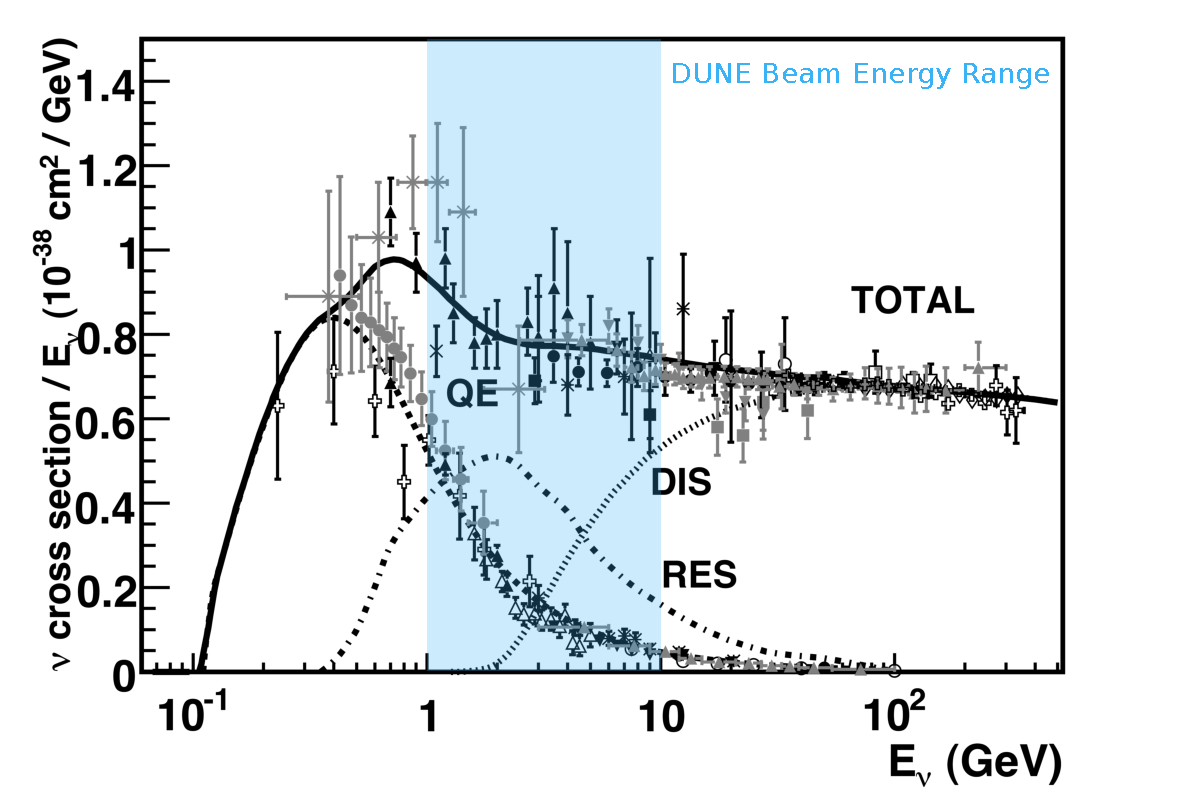
\includegraphics[width=\textwidth]{figures/numu_xsec.pdf}
	\caption
	[Muon neutrino cross section as a function of energy.]
	{Muon neutrino cross section per nucleon, per neutrino energy for an isoscalar
	target as a function of neutrino energy. The light blue region represents the 
	region of interest for the DUNE neutrino beam. Original figure from 
	\cite{Formaggio:2013kya}.}
	\label{fig:numu_xsec}
\end{figure}

The array of interaction modes available in DUNE means that there are many
particles which can be produced in the final state; understanding 
the composition of the final state is essential to the neutrino oscillation 
analysis. Part of this thesis, Chapter \ref{ch:chargeid}, looks at
the identification of charge deposits in a LArTPC. The results provide input 
in analyses of \protodune{} data, and the methods used could be adapted and 
developed for application in DUNE. 

\section{Supernova Neutrinos} \label{nu_sn}

Supernovae are extremely violent explosions, which are undergone by certain 
types of stars at the end of their life. These explosions can emit on the 
order of $10^{46}$ Joule of energy, and in certain cases, known as 
core--collapse supernovae, about 99\% of this energy is carried away by 
neutrinos.  Measurements of these neutrinos can provide insight into the 
mechanism involved in supernova bursts, as well as the study of neutrino 
masses\cite{GiuntiCarlo2007FoNP}.  

\subsection{Core--collapse Supernova Dynamics}

Core--collapse supernovae occur in stars with masses of around 10--60 solar 
masses. These stars will have undergone all stages of nuclear fusion during
their life, but since iron is the most tightly bound nucleus there is no fuel 
left to burn after it has been produced. At this stage, the iron core of the
star, which has a mass of around 1 solar mass, begins to collapse as the
pressure produced by nuclear fusion is no longer enough to counter the force of
gravity. 

During the collapse of the core, electron neutrinos are produced through
electron capture on both nuclei and free protons,
\begin{align*}
	e^- + N(Z, A) &\rightarrow N(Z - 1, A) + \nu_e \\
	e^- + p &\rightarrow n + \nu_e.
\end{align*}
At first, the mean free path of these neutrinos is much longer than the size of
the core, and the neutrinos leave the core carrying away their energy. This phase
of the collapse is known as the infall phase, it lasts on the order of 10ms and
releases neutrinos with energies of around 12--16 MeV.

Once the density of the core increases beyond around $3\times10^{11} \mbox{g 
cm}^{-3}$ neutrinos become trapped in the core, as the cross section for 
coherent scattering becomes large enough to prevent neutrinos from passing 
through the core. Neutrinos are still being produced by capture processes at 
this point, but they are unable to leave the core.

The core--collapse comes to a sudden halt about 1 second after it begins, when 
the density of the inner core reaches that of nuclear matter. At this stage, 
the core settles into equilibrium as a proto--neutron star while a shock--wave 
caused by this sudden halt propagates out through the layers of the star.  
Behind the shock, neutrino production is accelerated as nuclei are dissociated 
and the free protons capture electrons. Neutrinos begin to build--up behind 
the opaque shock. A few milliseconds after the bounce, the shock reaches a 
region of low enough density and becomes transparent, releasing the build--up 
of neutrinos in just a few milliseconds, this is known as the neutronisation 
burst.

One aspect of supernova dynamics, which is still unclear, is the so--called 
revival of the shock. As the shock dissipates through nucleon dissociation and 
neutrino emission it becomes weakened and eventually stalls around 100 ms 
after the initial bounce. During this time, known as the accretion phase, matter 
falls onto the collapsed core. If the shock cannot be revived a supernova will 
not occur. It is thought that neutrino flux produced in the proto--neutron 
star is able to revive the shock but the precise mechanics of this revival are 
still unknown. Studies have shown that the impact of spherical asymmetries 
might play an important role in allowing the burst to take 
place\cite{Tamborra:2014aua}. 

After the neutronisation burst, the main source of neutrino production comes 
from the proto--neutron star. Neutrinos of all flavours are produced in the 
core at a temperature of around 40 MeV. The release of neutrinos at this 
stage, known as the neutrino cooling phase, is significantly slower than that 
of the neutronisation burst and can last tens of seconds. During this phase, 
much like photons within a star, the neutrinos are mostly contained within the 
opaque environment of the proto--neutron star. They can only escape if they 
travel far enough from the core to a region where the opacity is sufficiently 
low. This region is called the neutrinosphere, it depends on flavour, and it 
is different for neutrinos and anti--neutrinos. These differences result in 
different energy distributions for each neutrino type, owing to the relative 
temperature of the star at the radius of each neutrinosphere,
\begin{align*}
	\langle E_{\nu_e} \rangle &\approx 10 \mbox{MeV} \\
	\langle E_{\xoverline{\nu_e}} \rangle &\approx 15 \mbox{MeV} \\
	\langle E_{\nu_x} \rangle &\approx 20 \mbox{MeV}
\end{align*}
where $\nu_x \in \left[\nu_\mu, \xoverline{\nu_\mu}, \nu_\tau, \xoverline{\nu_\tau}\right]$.

\subsection{SN1987A}

The first, and currently only, experimental observation of neutrinos from a 
supernova burst occurred in 1987. A small number of low--energy neutrino 
events were detected in coincidence with a supernova burst from the Large 
Magellanic Cloud, referred to as SN1987A. Three neutrino detectors reported an 
excess of low energy events in coincidence with the supernova: Kamiokande--II, 
IMB, and Baksan\cite{Hirata:1987hu, PhysRevLett.58.1494, Loredo:2001rx}. These 
events were primarily produced by two types of interaction, inverse beta decay 
(IBD),
\begin{equation*}
	n + \nu_e \rightarrow p + e^+,
\end{equation*}
and elastic scattering,
\begin{equation*}
	\nu_e + e^- \rightarrow \nu_e + e^-.
\end{equation*}
For supernova neutrinos, the inverse beta decay cross section is significantly 
higher than that of elastic scattering, therefore, most events are likely to be
due to inverse beta decay.

\subsubsection{Kamiokande--II}
Kamiokande--II was a water Cerenkov detector containing 2.1 kt of water. A
significant increase in the rate of electron events with respect to background
was observed, for a 10 second window which is coincident with 
SN1987A\cite{Hirata:1987hu}. Around 12 events were observed, their time sequence
and amplitudes are shown in Figure \ref{fig:kami_1987}. Unfortunately, due to 
an inaccurate detector clock, the absolute time of these events is only 
accurate to about one minute and, therefore, a time coincidence check with the 
other neutrino observations cannot be made.

\begin{figure}
	\centering
	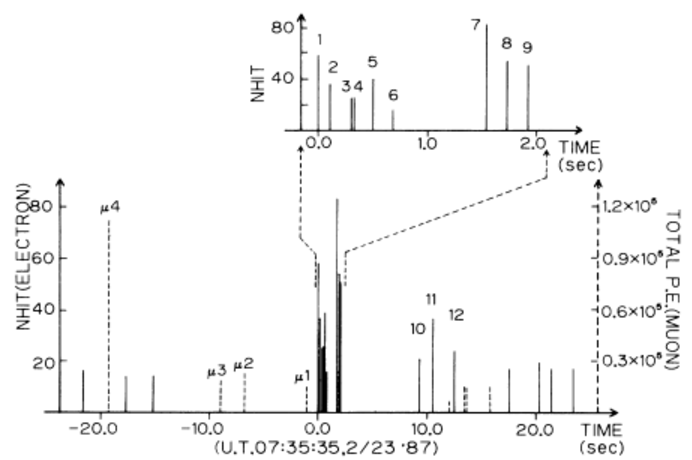
\includegraphics{figures/kami_1987.pdf}
	\caption
	[Measured supernova neutrino events from SN1987A in Kamiokande--II.]
	{Measured time of supernova neutrino events from SN1987A in Kamiokande--II. 
	Electron events are plotted as solid vertical lines, where the height of the 
	line represents the amplitude of the event in terms of number of PMT hits. 
	Muons are represented as dashed vertical lines, and the height of the line 
	represents the total number of measured photo--electrons. A clear excess of 
	electron events can be seen around the centre, this region is expanded above 
	the main axis of the figure. The supernova neutrino candidates are labelled
	with a number above the solid vertical line. Figure from 
	\cite{Hirata:1987hu}.}
	\label{fig:kami_1987}
\end{figure}

\subsubsection{IMB}
IMB was another water Cerekov detector, with a fiducial mass of 3.3 kt. They
observed eight neutrino candidate events, with energies in the range of 20--40
MeV within a six second window. The background rate was estimated to be around 2
events per day\cite{PhysRevLett.58.1494}.

\subsubsection{Baksan}
Unlike Kamiokande--II and IMB, the Baksan detector was a segmented liquid
scintillator detector with a total mass of around 330 tons. However, only a
limited fiducial mass of around 200 tons was used for the supernova neutrino
measurements. No excess above background could be observed by Baksan
in isolation, however, when input from Kamiokande--II and IMB is used, a 
cluster of 5 events within a 10s window was observed which coincided with the 
measurements from IMB\cite{Loredo:2001rx}.

\medskip\noindent
Since SN1987A, significant progress has been made for both experimental and
theoretical aspects of neutrino physics. Progress has been made in modelling
supernova explosions, and the impacts of neutrino oscillations on the supernova
environment have been considered\cite{Mirizzi:2015eza}. The current and next 
generation of neutrino experiments expect to measure thousands of neutrino 
events for a galactic supernova, instead of the tens measured by the previous
generation. The flux of neutrinos at earth has three components, $\nu_e$, 
$\xoverline{\nu_e}$, and $\nu_x$, the predicted energy spectra of each 
component is shown in Figure \ref{fig:sn_spec}.  Measuring the spectrum and 
time structure of a supernova neutrino burst could provide insights into the 
dynamics of supernovae, as well as neutrino physics.

\begin{figure}
	\centering
	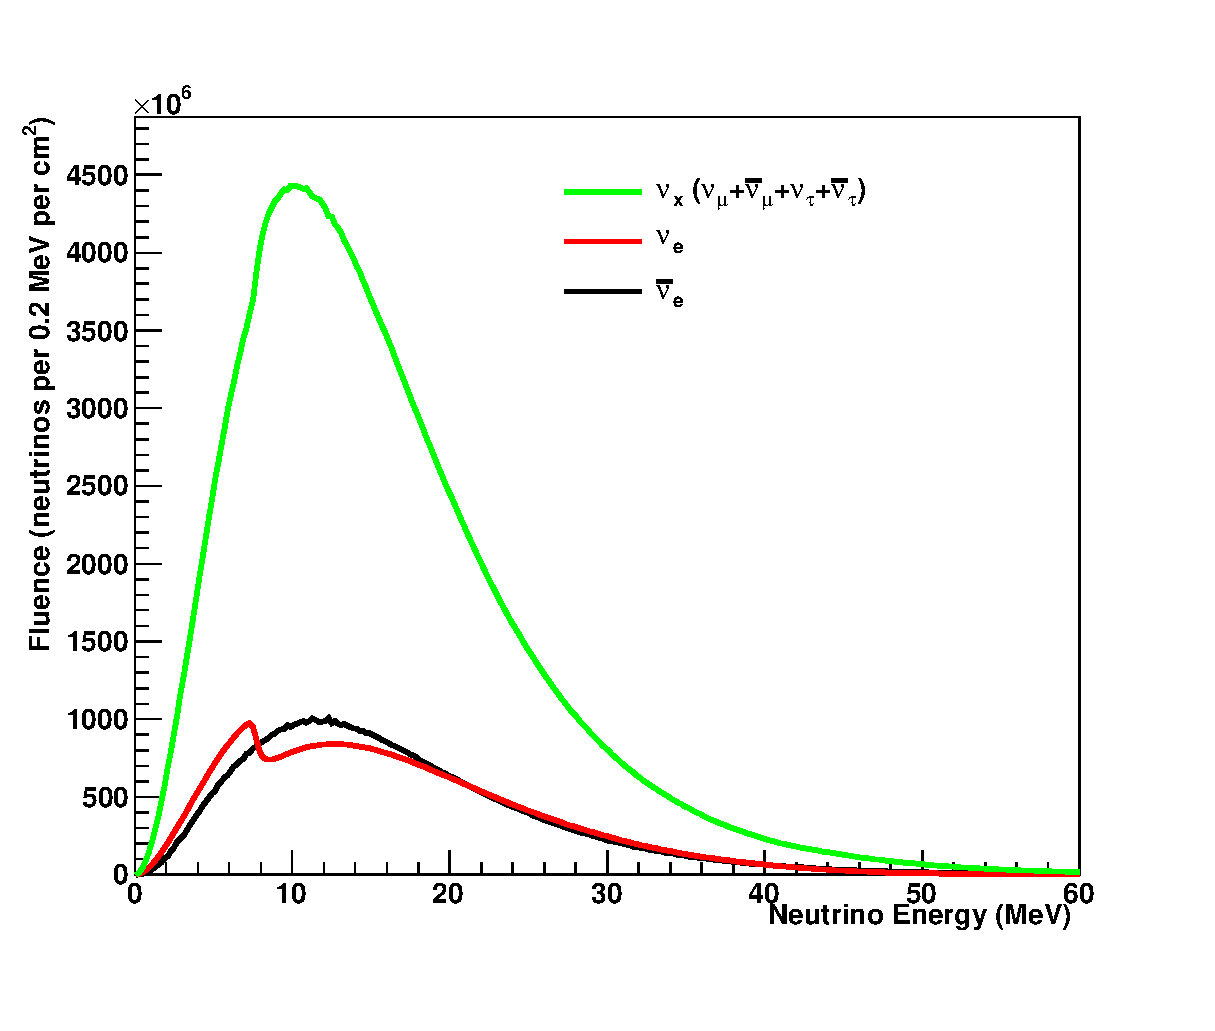
\includegraphics[width=\textwidth]{figures/supernova_spectrum_production.eps}
	\caption
	[Supernova neutrino flux at earth as a function of neutrino energy.]
	{Supernova neutrino flux at earth as a function of neutrino energy. The
	neutrino flux is split into three components, $\nu_e$, $\xoverline{\nu_e}$, 
	and $\nu_x$, which are plotted in red, black, and green respectively. Figure 
	from \cite{Scholberg:2012id}.}
	\label{fig:sn_spec}
\end{figure}

\subsection{Supernova Neutrino Prospects in DUNE}

The current world leading supernova neutrino detector is Super--Kamiokande, 
which expects to measure around 8000 events for a supernova at 10 
kpc\cite{Abe:2016waf}. As with Kamiokande--II, these events would primarily be 
produced via inverse beta decay interactions on the protons within the water.  
As such, Super--Kamiokande is mostly sensitive to the $\xoverline{\nu_e}$ 
component of the supernova neutrino flux. This is common amongst all water 
Cerenkov and scintillator based detectors, which make up the majority of the 
current landscape of supernova neutrino detectors. Therefore, DUNE makes a
highly complementary detector to the other supernova neutrino detectors, as a
result of the large CC cross section for $\nu_e$ on argon. In particular, 
DUNE offers a unique sensitivity to the neutronisation burst, which is 
primarily made up of $\nu_e$.  

\subsubsection{Supernova Neutrino Interactions in Liquid Argon}

Liquid argon should bring a strong sensitivity to the $\nu_e$ component of a
supernova neutrino burst, via the charged--current absorption of $\nu_e$ on
$^{40}\mbox{Ar}$,
\begin{equation*}
	\nu_e + ^{40}\mbox{Ar} \rightarrow e^- + ^{40}\mbox{K}^*.
\end{equation*}
This interaction leaves an $e^-$ and an excited $K$ in the final state. In 
addition, there are charged--current $\xoverline{\nu_e}$ interactions with 
argon, and elastic scattering interactions with electrons, which are available 
to neutrinos of all flavours. The dominant cross sections in liquid argon as a 
function of energy are shown in Figure \ref{fig:sn_xsec}\cite{Abi:2020evt}.

\begin{figure}
	\centering
	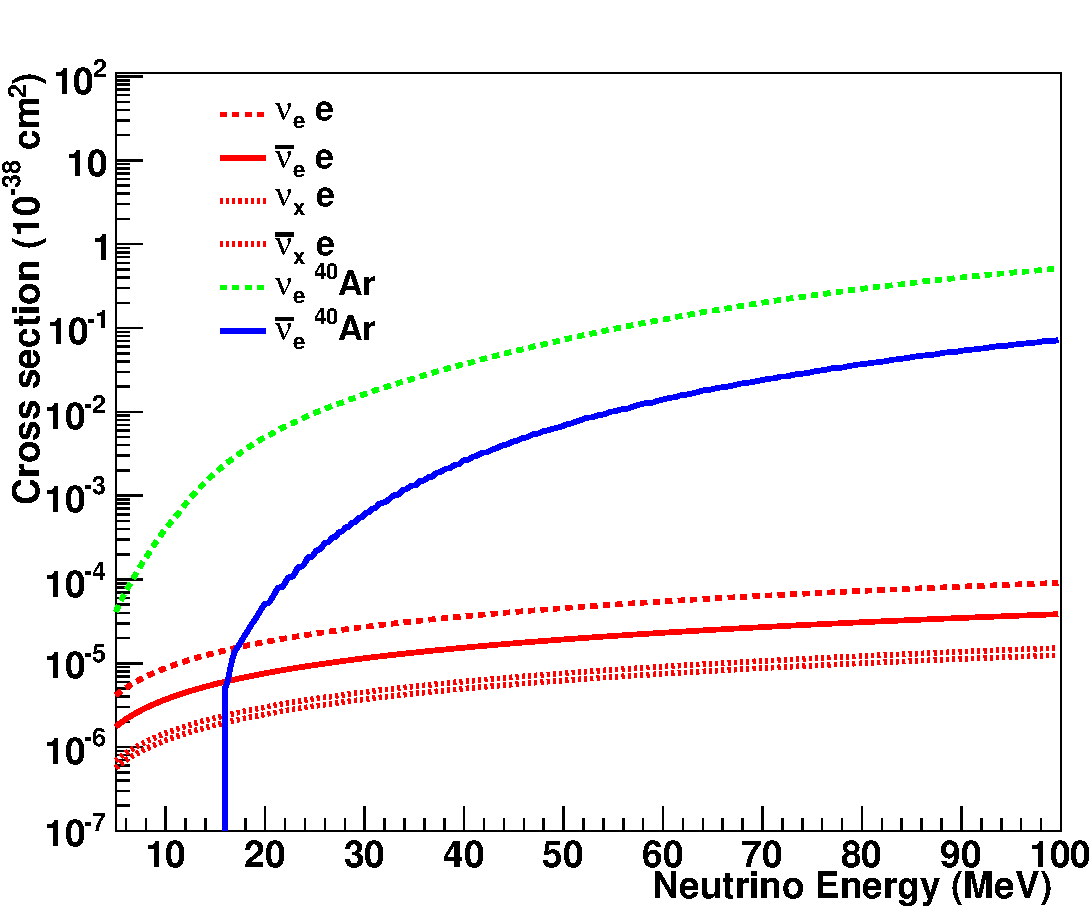
\includegraphics[width=\textwidth]{figures/sn_xsec.pdf}
	\caption
	[Neutrino cross sections in liquid argon as a function of neutrino energy, in
	the energy regime relevant for supernova neutrinos.]
	{Neutrino cross sections in liquid argon as a function of neutrino energy, in 
	the energy regime relevant for supernova neutrinos. The cross
	section is split into a number of components, depending of the properties of
	the neutrino and the target, which are labelled in the top left corner of the 
	figure. Figure from \cite{Abi:2020evt}.}
	\label{fig:sn_xsec}
\end{figure}

\subsubsection{Supernova Neutrino Events in DUNE}

For a 10 kpc supernova, DUNE expects to observe roughly 3000 neutrino events,
over a period of around 10 seconds. In DUNE, this will show up as a sudden
increase in the rate of low--energy electron events in the detector. Figure 
\ref{fig:sn_nus} shows the predicted time structure and energy spectrum for a 
simulated supernova event in DUNE\cite{Abi:2020evt}. The details of the rate 
and energy of these events as a function of time can hold potential insights 
into both neutrino physics and the dynamics of supernova bursts. 

\begin{figure}

	\centering

	\begin{subfigure}[b]{\textwidth}
		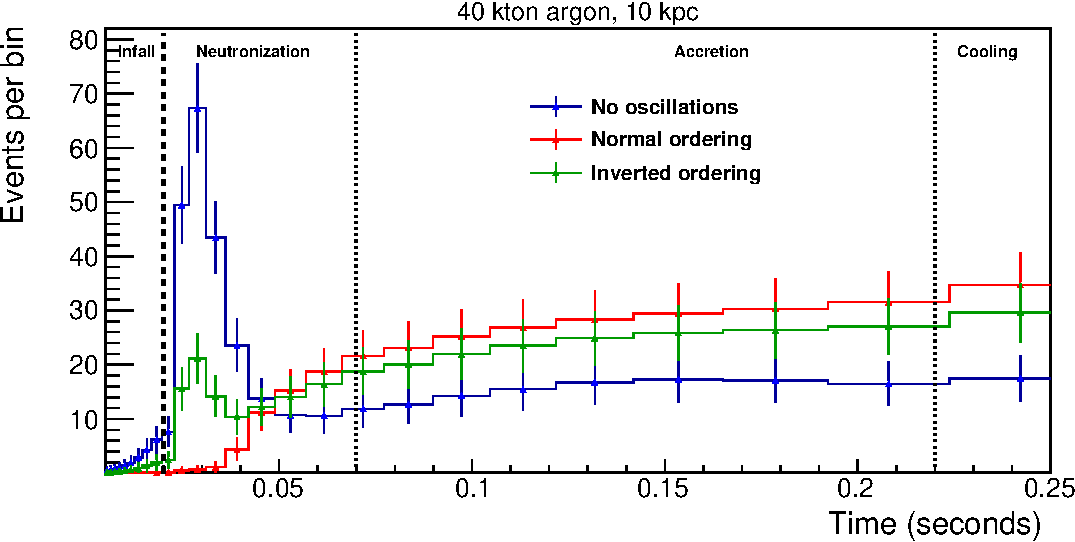
\includegraphics[width=\textwidth]{figures/sn_time.pdf}
		\caption {Observed event rate for the first 0.25 seconds of the supernova
		neutrino burst. The predictions under the assumption of no oscillations, 
		normal neutrino mass ordering, and inverted neutrino mass ordering are shown 
		in blue, red, and green respectively. Figure from \cite{Abi:2020evt}.}
		\label{fig:sn_time}
	\end{subfigure}

	\begin{subfigure}[b]{\textwidth}
		\centering
		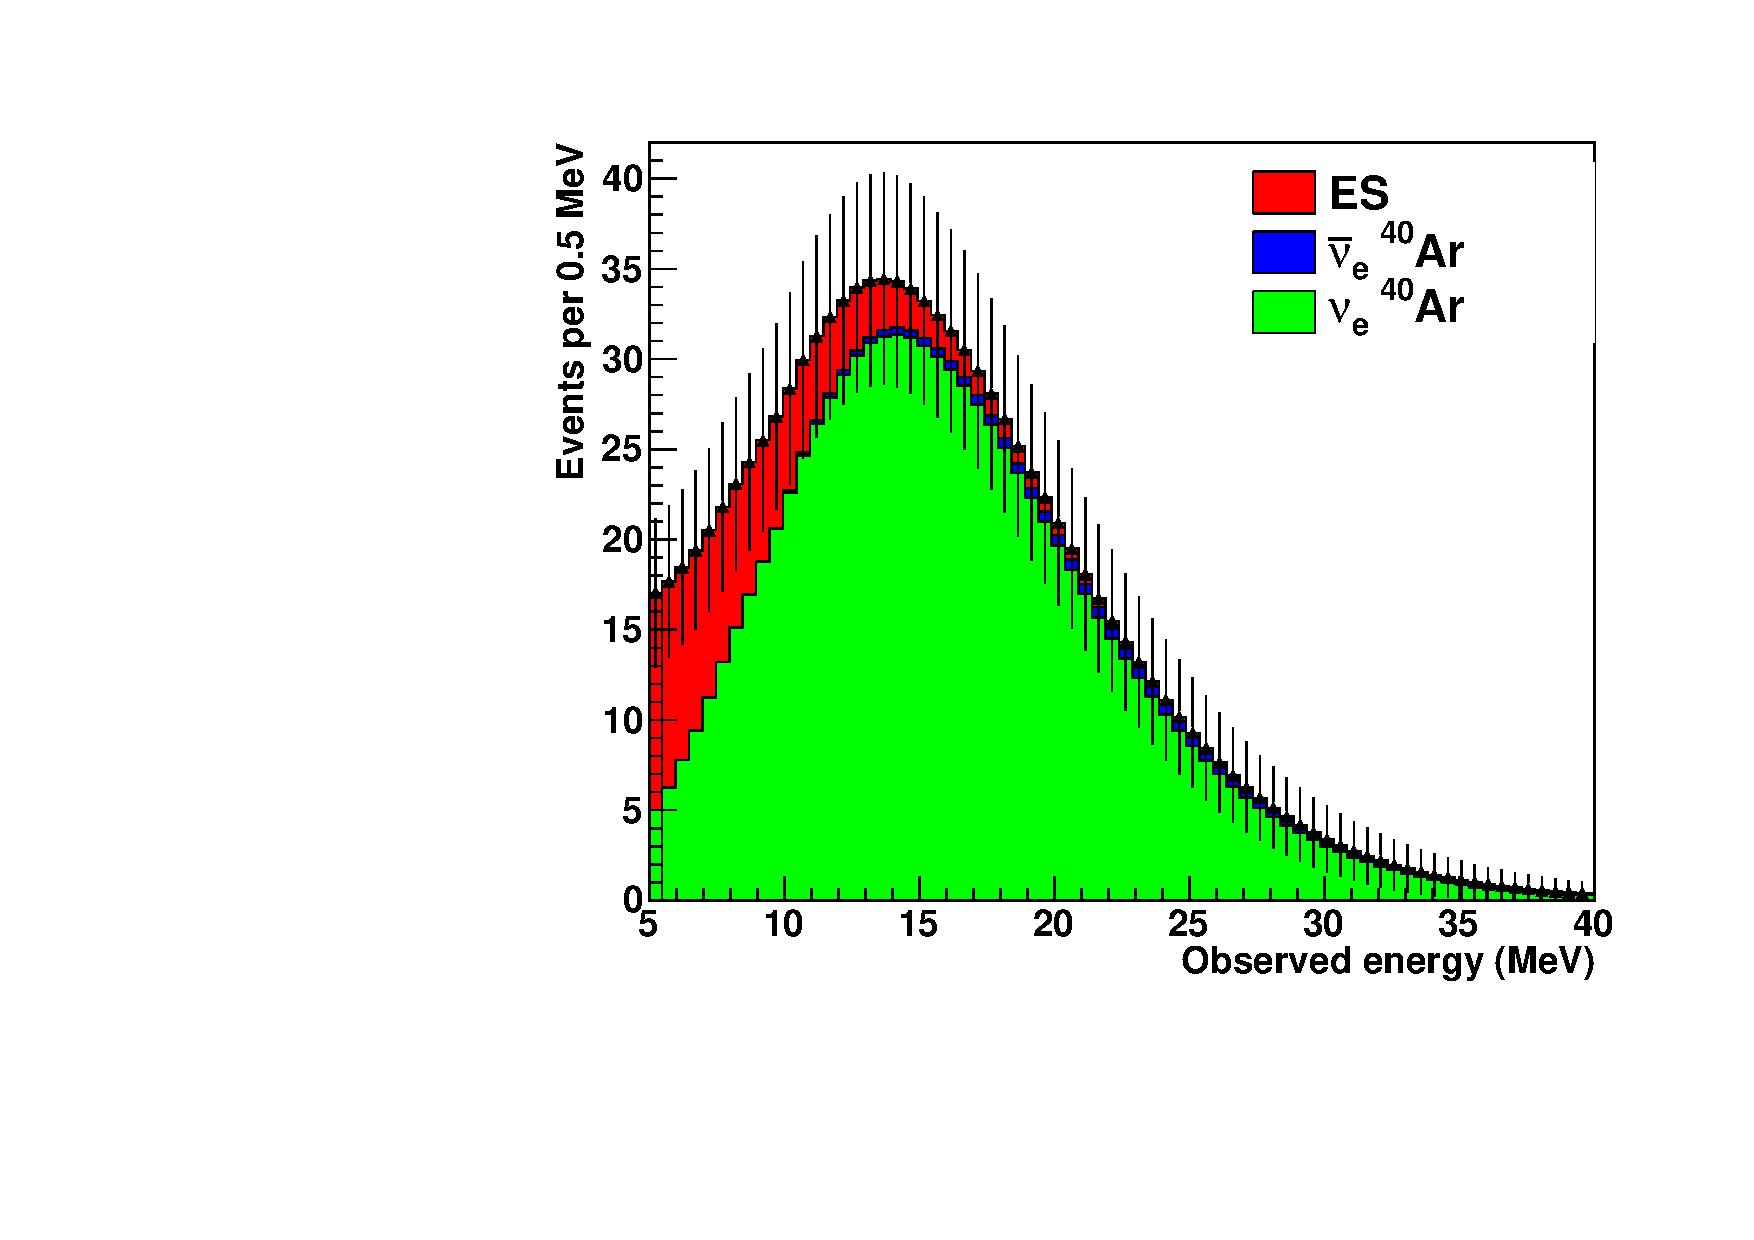
\includegraphics[width=0.9\textwidth]{figures/sn_energy.pdf}
		\caption {Observed supernova neutrino energy spectra for the full supernova
		neutrino burst. The contributions from elastic scattering,
		$\xoverline{\nu_e}$, and $\nu_e$ events are shown in red, blue, and green
		respectively. Figure from \cite{Acciarri:2015uup}.}
		\label{fig:sn_energy}
	\end{subfigure}

	\caption
	[Predicted supernova neutrino event rate and energy spectra for a 10 kpc
	core collapse supernova measured by DUNE.]
	{Predicted supernova neutrino event rate and energy spectra for a simulated 
	10 kpc core collapse supernova measured by DUNE.}

	\label{fig:sn_nus}

\end{figure}

Detecting and reconstructing tens of MeV electrons is necessary to study 
supernova neutrinos, as can be seen from the observed energy spectrum for 
supernova neutrinos in Figure \ref{fig:sn_nus}. There are significant 
challenges involved in this measurement as a result of the difficulties involved
in the detection of low energy activity and the reconstruction of low--energy 
electrons. Effectively reconstructing electrons in the tens of MeV range is 
essential to improving our understanding of supernova neutrinos in DUNE. This 
is discussed in Chapter \ref{ch:michel}, using the case of Michel electrons in 
\protodune{} to benchmark the performance of low energy electron reconstruction 
in liquid argon time projection chambers.
